% Simo.Nikula@gmail.com
% based on latex template at http://www.lut.fi/web/en/library/dissertations1 
\def\mytitle{Description of plasticity in physics engine}
\def\myisbn{978-952-265-XXX-X}
\def\mypdfisbn{978-952-265-XXX-X}
\def\myyear{2017}
\def\mymonth{May}
\def\myname{Simo Nikula}
\def\lut{Lappeenranta University of Technology}
\def\bullet{Bullet Physics}
\def\demolisher{DemolisherDemo}
\def\charpy{CharpyDemo}
\documentclass[a4paper,twoside,12pt,notitlepage]{article}
\usepackage[utf8]{inputenc}
\usepackage{graphicx}
\usepackage{natbib}
\usepackage{lastpage}   % page count
\usepackage{amsmath}
\usepackage{listings}
% \usepackage{mathdots}  % improved \ddots and \iidots
\usepackage{amssymb}
\usepackage[english]{babel}
\usepackage[intoc]{nomencl} % including table of content
\usepackage{ifthen}
\usepackage[hmargin=2.0cm,vmargin=1.6cm]{geometry} % setting marginals
\usepackage{fancyhdr,extramarks}  % header ja footer manipulation
\usepackage{times}  % to change font to times
\usepackage{setspace} % for linespacingx
\usepackage{tikz}
\usetikzlibrary{arrows}
\usetikzlibrary{arrows.meta}
\usepackage{caption}
\usepackage{varwidth}
\usepackage{enumitem} % 
\newcommand{\nomunit}[1]{\renewcommand{\nomentryend}{\hspace*{\fill}#1}} % Inserts units on the right at symbol list
\renewcommand{\nomgroup}[1]{%
 \ifthenelse{\equal{#1}{C}}{\item[\textbf{Latin alphabet}]\item}{%
 \ifthenelse{\equal{#1}{G}}{\item\item[\textbf{Greek alphabet}]\item}{}}{%
 \ifthenelse{\equal{#1}{L}}{\item\item[\textbf{Subscripts}]\item}{}}{%
 \ifthenelse{\equal{#1}{H}}{\item\item[\textbf{Superscripts}]\item}{}}{%
 \ifthenelse{\equal{#1}{W}}{\item\item[\textbf{Abbreviations}]\item}{}}{}}

\singlespacing

\pagestyle{fancy}
\fancyhf{}% clearing the header and footer
\fancyhead[LE,RO]{\bfseries\thepage}    % page number to header
\fancyhead[LO]{\nouppercase{\bfseries\rightmark}}     %
\fancyhead[RE]{\nouppercase{\bfseries\leftmark}}%

\renewcommand\sectionmark[1]
 {\markboth{\thesection\ #1}{}}         % section name to header
\renewcommand\subsectionmark[1]
 {\markright{\thesubsection\ #1}}       % subsection name to header
\renewcommand{\headrulewidth}{0.5pt}    % ruler thickness between head and body
\renewcommand{\footrulewidth}{0pt}      % no ruler between body and footer

\setlength{\nomitemsep}{-\parsep}   % removing default extra skip between entries at nomenclature

\numberwithin{equation}{section}    % equation numbers with section numbers
\numberwithin{table}{section}       % table numbers with section numbers
\numberwithin{figure}{section}      % figure numbers with section numbers

% makeindex command needs to run at command prompt to create nomenclature list file
\makenomenclature % makeindex main_v2.nlo -s nomencl.ist -o main_v2.nls
%\bibpunct{(}{)}{;}{a}{,}{,}%

\begin{document}

\pagestyle{empty}
\title{\mytitle}
\author{Simo Nikula, Aki Mikkola and Timo Björk}
\author{}
\maketitle
\section{Introduction}

Physics engine is computer software that provides an approximate simulation of physical system. 
E.g. ODE - \cite{ode}, \bullet - \cite{bullet}, Box2D - \cite{box2d} are open source physics engines that are  widely used in 
areas where fast solutions are required. Typical industries are games and film productions.

Computational methods used in physics engines are divided to modules that handle collision detection and modules that handle simulation.
Simulation can further be subdivided into time control, motion solver, constraint solver and collision solver modules.
Velocity-based formulation is used in constraint based rigid body simulation frameworks as collisions cannot be handled easily in acceleration based formulations. Friction is typically taken into account. Joints are handled by constraint equations.
Detailed description of various components  can be found in e.g. \cite{erleben.thesis}.
In this work focus is on solving new types of joints between rigid objects.

Plasticity is not typically taken into account in gaming solutions. 
Breaking of various objects typically takes place based on collision or impulse and breaking of steel or 
reinforced concrete structures does not look realistic.
Theory for handling of plasticity has been presented already in \cite{cg1988}. 
\cite{muller2004point} presents a method for modeling and animating of elastic and plastic objects in realtime using point based animation but it is not widely used.

Goal of this work is to find method that can be used in widely used physics engines to make simulation more realistic
by connecting rigid objects by  spring based constraints which have additional properties for handling plasticity.
Main target is that plastic deformation takes place if force or moment exceeds given limit, deformation absorbs energy and 
joint breaks if plastic capacity is exeeced.

Methods presented in this work can be used in gaming industry to provide more realistic simulations without significant extra work. 
For gaming purposes presented method works best in scenarios where connected parts are relatively heavy. 
This allows normal integration timestep to be used without stability issues.
This kind of metodology also opens quite large area of combining old structural analysis methods to modern simulation frameworks.

% !TeX root = article.tex
\section{Description of plasticity in the framework of physics engines}

In this section, key concepts related to the introduced model are explained. The main differences between 
traditional structural analysis and physics engines based approaches are reviewed and discussed.

Velocity-based formulation is  commonly used by physics based game
developers and film production teams.
%\citet[p.~45]{erleben.thesis} 
\citet{erleben.thesis} 
provides reasoning and theoretical details for the popularity of 
velocity-based formulation in constraint-based rigid body simulation. 
The main reason is that collision handling can be done without the use of additional procedures.

Work presented by  
\citet{erleben.thesis} provides the basis for the velocity-based formulation discussed in this work.
%\citet[p.~45-50]{erleben.thesis}.
% pdf page 64
In following section, these formulations will be clarified by simple example using \bullet\ implementation.

Impulse $\vec{J}$
in the time interval $\Delta t $ can we written as
\begin{equation} \label{eq:impulseIntegral}
\vec{J} = \int_{0}^{\Delta t} \vec{f}_{true}(t) dt,
\end{equation}
where $\vec{f}_{true}(t)$ is force.

Newton's second law of motion $\vec{F}=m\vec{a}$ one can solve for the velocity,
$\vec{v}^{\Delta t}$ as
\begin{equation} \label{eq:impulseIntegraWithNewton}
\int_{0}^{\Delta t} m \frac{d\vec{v}}{dt}dt= \int_{0}^{\Delta t} \vec{f}_{true}(t)
\end{equation}
\begin{equation} \label{eq:impulse}
m(\vec{v}^{\, \Delta t} - \vec{v}^{\, 0})=\vec{J}
\end{equation}
where superscripts denote time, i.e. ${\vec{v}}^{\Delta t}=\vec{v}(\Delta t)$.
Next position can be found
by integrating the velocity.
Updates after each step can be summarized  for locations and  
for velocities correspondingly as follows.

\begin{equation} \label{eq:eomL} % pdf page 69
\vec{s}^{\, t+\Delta t} = \vec{s}^{\, t}+\Delta t S \vec{u}^{\, t+\Delta t}
\end{equation}

\begin{equation} \label{eq:eomV}
\vec{u}^{\, t+\Delta t} = \vec{u}^{\, t}+\Delta t M^{-1}(C N \vec{f}^{\ t+\Delta t} + \vec{f}_{ext}) 
\end{equation}

Symbols used in Equations \ref{eq:eomL} and \ref{eq:eomV}
are summarized in Table \ref{tab:eom} and Figure \ref{fig:eom-contact}.
Figure \ref{fig:eom-contact} describes collision of two bodies $B_1$ and $B_2$

\begin{figure}[htb!]
\centering
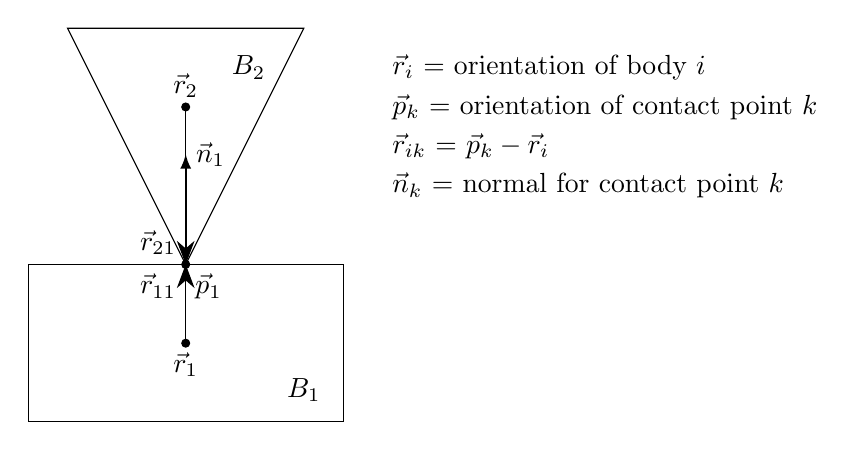
\begin{tikzpicture}
\coordinate (O1) at(2,1);
\coordinate (O2) at(2,4);
\coordinate (C) at(2,2);
\draw (0,0) -- (4,0) -- (4,2) -- (0,2) --(0,0);
\draw (2,2) -- (3.5,5) -- (0.5,5) -- (2,2) ;
\node at (3.5,0.4) {$B_1$};
\filldraw (O1) circle (0.5mm) node[anchor=north] {$\vec{r}_1$};
\node at (2.8,4.5) {$B_2$};
\filldraw (O2) circle (0.5mm) node[anchor=south] {$\vec{r}_2$};
\filldraw (C) circle (0.5mm) node[anchor=north west] {$\vec{p}_1$};
\draw[-{Stealth[length=3mm]}] (O1) -- (C) node[anchor=north east] {$\vec{r}_{11}$};
\draw[-{Stealth[length=3mm]}] (O2) -- (C) node[anchor=south east] {$\vec{r}_{21}$};
\draw[-latex,thick] (C) -- ++(0,1.4) node[anchor=west] {$\vec{n}_{1}$};
\node[anchor=west] at (4.5,4.5) {
$\vec{r}_i$  =  orientation of body $i$
};
\node[anchor=west] at (4.5,4) {$\vec{p}_k $ = orientation of contact point $k$};
\node[anchor=west] at (4.5,3.5) {$\vec{r}_{ik} $ = $\vec{p}_k - \vec{r}_i $};
\node[anchor=west] at (4.5,3) {$\vec{n}_{k} $ = normal for contact point $k$};
\end{tikzpicture}
\caption{Illustration of nomenclature for equations of motion for contact.}
\label{fig:eom-contact}
\end{figure}

where $\vec{r}_i$ is orientation of body $i$,
$\vec{p}_k $ is orientation of contact point $k$,
$\vec{r}_{ik} $ is vector  between center of gravity of body $i$ and contact point $k$
and
$\vec{n}_{k}$ is contact normal for contact point $k$.
By employing this formulation, simplified scenario can be simulated.


% pdf page 33, notation in typical ODEs
\begin {table}[htb!]
\caption {Nomenclature for equations of motion}
\label{tab:eom}
\begin{center}
\begin{tabular}{|l| l|}
\hline
{\bf Symbol} & {\bf Description} \\  \hline
$\vec{r}_i$ & position of center of mass for body $i$  \\ \hline
$\vec{q}_i$ & orientation for body $i$ as quaternion $\lbrack s_i, x_i, y_i, z_i \rbrack ^T $ \\
\hline
$\vec{p}_h$ & contact or joint point $k$  \\ \hline
$\vec{r}_{ki}$ & $\vec{p}_k - \vec{r}_i$  \\ \hline
$\vec{s}$ & $\lbrack \vec{r}_1, \vec{q}_1,...,\vec{r}_n, \vec{q}_n \rbrack ^T $\\ \hline
$Q_i$ & \begin{tabular}{@{}c}
rotation of quaternion $\vec{q}_i$
as matrix \\ where 
$\frac{1}{2}\vec{\omega}_i \vec{q}_i=Q_i \vec{\omega}_i$
\end{tabular}
   $
\frac{1}{2} \left[ \begin{array}{ccc}
-x_i & -y_i & -z_i \\
s_i & z_i & -y_i \\
-z_i & s_i & x_i \\
y_i & -x_i & s_i
\end{array} \right]
$
\\ \hline
$S$ & 
\begin{tabular}{@{}c}
generalized transformation matrix \\
$ S \in \mathbb{R}^{7n \times 6n}$
\end{tabular}
 $ \left[ \begin{array}{ccccc}
1 &  &  & & 0 \\
 & Q_i  \\
 & & \ddots  \\
 & & & 1 \\
0 & & & & Q_n 
\end{array} \right]
$
\\ \hline
$\vec{v}_i$ & linear velocity of  center of mass for body $i$   \\ \hline
$\vec{\omega}_i$ & angular velocity of center of mass for body $i$  \\ \hline
$\vec{u}$ & $\lbrack \vec{v}_1, \vec{\omega}_1,...,\vec{v}_n, \vec{\omega}_n \rbrack ^T $\\ \hline
$M$ &
\begin{tabular}{@{}c}
 generalized mass matrix \\
$ M \in \mathbb{R}^{6n \times 6n}$  
\end{tabular}
$
\left[ \begin{array}{ccccc}
m_i 1 &  &  & & 0 \\
 & I_1  \\
 & & \ddots  \\
 & & & m_n 1 \\
0 & & & & I_n 
\end{array} \right]
$
\\ \hline
$I_i$ & inertia tensor for body $i$  \\ \hline
$C$ & contact condition matrix  $ C \in \mathbb{R}^{6n \times 3K}$ \\ \hline
$N$ & contact normal matrix  $ N \in \mathbb{R}^{3K \times K}$ \\ \hline
\end {tabular}
\end{center}
\end {table}

Friction in contacts and joint constraints can be handled in unified way by refactoring
equation \ref{eq:eomV} as,  
\citet{erleben.thesis}
%\citet[p.~66-67]{erleben.thesis}
\begin{equation} \label{eq:eomV2}
\vec{u}^{\, t+\Delta t} = \vec{u}^{\, t}+\Delta t M^{-1}(
 J_{contact}^T \vec{\lambda}_{contact}
+ J_{joint}^T \vec{\lambda}_{joint}
+ \vec{f}_{ext})
\end{equation}

where jacobian terms $J_{contact}^T$ for joints are 
derived by taking time derivates of kinematic constraints.

Symbols used in Equation \ref{eq:eomV2} are summarized in Table
\ref{tab:eom-g} and Figure \ref{fig:eom-joint}.
Figure \ref{fig:eom-joint} shows terms needed for joint processing.

\begin{figure}[htb!]
\centering
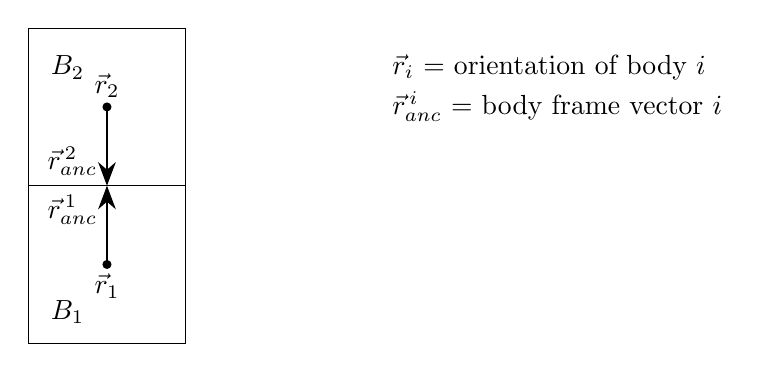
\begin{tikzpicture}
\coordinate (O1) at(1,1);
\coordinate (O2) at(1,3);
\coordinate (C) at(1,2);
\draw (0,0) -- (2,0) -- (2,2) -- (0,2) --(0,0);
\draw (0,2) -- (2,2) -- (2,4) -- (0,4) --(0,2) ;
\node at (0.5,0.4) {$B_1$};
\filldraw (O1) circle (0.5mm) node[anchor=north] {$\vec{r}_1$};
\node at (0.5,3.5) {$B_2$};
\filldraw (O2) circle (0.5mm) node[anchor=south] {$\vec{r}_2$};
\draw[-{Stealth[length=3mm]}] (O1) -- (C) node[anchor=north east] {$\vec{r}_{anc}^{\,1}$};
\draw[-{Stealth[length=3mm]}] (O2) -- (C) node[anchor=south east] {$\vec{r}_{anc}^{\,2}$};
\node[anchor=west] at (4.5,3.5) {
$\vec{r}_i$  =  orientation of body $i$ 
};
\node[anchor=west] at (4.5,3) {$\vec{r}_{anc}^{\,i} $ = body frame vector $i$};
\end{tikzpicture}
\caption{Illustration of nomenclature for equations of motion for joint.}
\label{fig:eom-joint}
\end{figure}

In Figure \ref{fig:eom-joint}, $\vec{r}_{anc}^{\,i}$ is used to define at which point
joint constraint is applied.

% pdf page 33, notation in typical ODEs
\begin {table}[htb!]
\caption {Additional terms  for generalized equations of motion}
\label{tab:eom-g}
\begin{center}
\begin{tabular}{|l| l|}
\hline
{\bf Symbol} & {\bf Description} \\  \hline
$J_{contact}$ & Jacobian matrix for contacts  \\ \hline
$\lambda_{contact}$ & vector of lagrange multipliers for contacts  \\ \hline
$J_{joint}$ & Jacobian matrix for joints  \\ \hline
$\lambda_{joint}$ & vector of lagrange multipliers for joints  \\ \hline
\end {tabular}
\end{center}
\end {table}

Constraint processing in \bullet\ is based on ODE, \cite{ode}.
Joints are also discussed in detail in  
\citet{erleben.thesis}.
%\citet[p.~60-90]{erleben.thesis}.
Equations \ref{eq:constraintEquation}, \ref{eq:lambdaLow} and
\ref{eq:lambdaHigh} 
are created for each constraint. 
Derivation for terms in Equation \ref{eq:constraintEquation}
can be done using position and orientation of connected bodies.
E.g. for ball joint formulation is based on both joint points having same position.
In contact cases formulation is easier if it is done using velocities, \cite{ode.joints}.

\begin{equation} \label{eq:constraintEquation}
J_1 \vec{v}_1 + \Omega_1 \vec{\omega}_1 + 
J_2 \vec{v}_2 + \Omega_2 \vec{\omega}_2 = \vec{c} + C \vec{\lambda}
\end{equation}

\begin{equation} \label{eq:lambdaLow}
\vec{\lambda} \geq \vec{l}
\end{equation}

\begin{equation} \label{eq:lambdaHigh}
\vec{\lambda} \leq \vec{h}
\end{equation}

In following section, these equations will be clarified by simple example.
Main parameters  and corresponding fields in \bullet\  
 are described in Table \ref{tab:constraintParameters}.

\begin {table}[htb!]
\caption {Constraint parameters}
\label{tab:constraintParameters} 
\begin{center}
\begin{tabular}{|c| l| l|}
\hline
{\bf Parameter} & {\bf Description} & {\bf btConstraintInfo2 pointer}\\  \hline
$J_1, \Omega_1$ & jacobian & m\_J1linearAxis, m\_J1angularAxis \\
$J_2, \Omega_2$ & & m\_J2linearAxis, m\_J2angularAxis \\ \hline
$\vec{v}$ & linear velocity & \\ \hline
$\vec{\omega}$ & angular velocity & \\ \hline
$\vec{c}$        &  right side vector   & m\_constraintError \\ \hline
$C$  & constraint force mixing & cfm \\  \hline
$\vec{\lambda}$ & constraint force &  \\ \hline
$\vec{l}$ & low limit for constraint force & m\_lowerLimit \\ \hline
$\vec{h}$ & high limit for constraint force & m\_upperLimit \\ \hline
\end {tabular}
\end{center}
\end {table}


In structural analysis, a formulation and associated numerical solution procedure are selected 
based on needed features.
Often,  finite element method is used.
In most cases, static solution with assumption of linear strain-displacement relation
using displacement based boundary conditions is used.
\citet{bathe-1975} provides description for handling of various nonlinearities.
In large displacement analysis, formulation may be based on updated formulation (Eulerian) or
Lagrangian formulation where initial configuration is used.
Further enhancements are material nonlinearity and dynamic analysis.
Physics engine provides dynamic analysis with large reference translations and rotations
while assuming bodies to be undeformable.

Material plasticity can be accounted in games by using suitable coefficient of restitution.
This provides reasonable means to simulate loss of energy in collisions.
Simulation of breaking of bodies made of ductile material can be made more realistic by splitting rigid body
to multiple bodies which are connected by energy absorbing joints.
Typical engineering stress-strain curve of ductile steel is shown in Figure \ref{fig:sscurve}.

\begin{figure}[htb!]
\centering
\begin{tikzpicture}
\coordinate (Y) at (1,4);
\draw[->] (0,0) -- (10,0) node[right] {\large{$\epsilon$}};
\draw[->] (0,0) -- (0,6) node[above] {\large{$\sigma$}};
\draw(0,0) -- (Y) -- (2,4) .. controls (7,6) .. (10,5);
\draw[dashed](0,4) -- (Y);
\node at (-0.2,4) [align=right] {$f_y$};
\draw(0.25,1) -- (0.5,1) -- (0.5,2);
\node at (0.75,1.5) {$E$};
\node at (0.8,2.5) [anchor=west] {$\sigma = E \epsilon$ if $\sigma \le f_y$};
\end{tikzpicture}
\caption{Engineering stress-strain curve of ductile steel (not to scale).}
\label{fig:sscurve}
\end{figure}

In Figure \ref{fig:sscurve}, $\sigma$ is stress, $E$ is Youngs modulus and $f_y$ is yield stress.
Engineering stress and strain mean that original dimensions are used in stress calculation,
\citet{dowling}.
%\citet[p.~108]{dowling}.
Stress-strain curve is not drawn to scale as elastic strain could not be seen as it is typically 0.001 to 0.005.

In this work elastic-fully plastic material model is used in most scenarios.
Having elastic part allows elastic displacements for slender structures. 
Elastic material behavior is ignored in approach introduced in this work provided
that deformation is related to higher frequency
than integration stability would allow.
It should be noted that geometry
of bodies is not updated during analysis and thus engineering stress-strain properties should
be used.

In this work, strain hardening is taken into account by assuming that plasticity in bending
expands, 
\citet{dowling}.
%\citet[p.~672]{dowling}.
Material that starts to yield first is hardened and as a result of which yielding moves.
This can be seen e.g. by bending paperclip. It does not break at low angles but can take few full bends. 

Difference between elastic and plastic section modulus is depicted in Figure \ref{fig:wp}.

\begin{figure}[htb!]
\centering
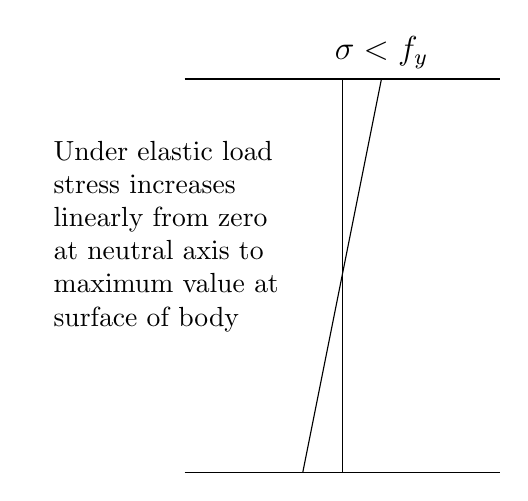
\begin{tikzpicture}
\coordinate (S) at (2.5,5);
\draw (0,5) -- (4,5) ;
\draw (0,0) -- (4,0) ;
\draw (2,0) -- (2,5) ;
\draw (1.5,0) -- (S); 
\node[above] at (S) [align=center] {\large{$\sigma<f_y$}};
\node[anchor=west] at (-2,3) {
\begin{tabular}{l}
Under elastic load\\
stress increases\\
linearly from zero\\
at neutral axis to\\
maximum value at \\
surface of body
\end{tabular}
};
\end{tikzpicture}
\hspace{1cm}
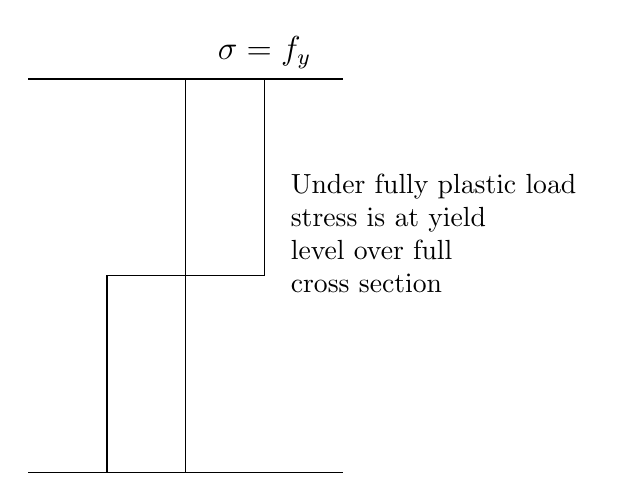
\begin{tikzpicture}
\coordinate (S) at (3,5);
\draw (0,5) -- (4,5) ;
\draw (0,0) -- (4,0) ;
\draw (2,0) -- (2,5) ;
\draw (1,0) -- (1,2.5) -- (3,2.5) -- (S); 
\node[above] at (S) [align=center] {\large{$\sigma=f_y$}};
\node[anchor=west] at (3,3) {
\begin{tabular}{l}
Under fully plastic load\\
stress is at yield\\
level over full\\
cross section
\end{tabular}
};
\end{tikzpicture}
\caption{Axial stress distribution over cross section for bending under elastic and fully plastic loads.}
\label{fig:wp}
\end{figure}

As shown in Figure 2.4, if stress is below yield limit $f_y$, stress and strain are linear within material.
If cross section is fully plastic, stress is assumed to be at yield level over whole cross section such that 
plastic section modulus is higher than elastic section modulus.

In this work, plasticity is handled by defining maximum forces
in Equations \ref{eq:lambdaLow} and  
\ref{eq:lambdaHigh} using plastic capasities which are defined below.

Maximum force acting in a direction of $\vec{r}_{anc}^{\,i} $
is product of area and yield stress as follows

\begin{equation} \label{eq:fN}
N_{max}= \int_A f_y
\end{equation}

Maximum forces acting perpendicular to $\vec{r}_{anc}^{\,i} $
are product of area and shear yield stress $\tau_y$ as follows
\begin{equation} \label{eq:fQ}
Q_{max}= \int_A \tau_y
\end{equation}

Maximum moments acting around axis perpendicular to $\vec{r}_{anc}^{\,i} $
are integrals of perpdendicular distance 
and yield stress $f_y$ as given for the moment around $x$-axis 
and moment around $z$-axis, respectively.

\begin{equation} \label{eq:Mx}
M_{max}^x= \int_A z f_y
\end{equation}

\begin{equation} \label{eq:Mz}
M_{max}^z= \int_A x f_y
\end{equation}

Maximum moment around $\vec{r}_{anc}^{\,i} $
is integral of distance $d$ from joint point
and shear yield stress $\tau_y$ as 

\begin{equation} \label{eq:My}
M_{max}^y= \int_A d \tau_y
\end{equation}

Maximum forces and moments for 
rectangular section with width $b$ and height $h$ using constant yield stress
are summarized in Table \ref{tab:maxForces}.
Yield shear stress is assumed to be $ 0.5\, f_y$ using Tresca yield critetion.
If von Mises yield criterion is used 0.5 is replaced by 0.58 ($1/\sqrt{3}$), \cite{dowling}.
% p. 262, p. 268
These are not exact values in multiaxial stress state but they
are usable in most cases.


\begin {table}[htb!]
\caption {Maximum forces and moments for 
rectangular section with width $b$ and height $h$ using constant yield stress $f_y$}
\label{tab:maxForces} 
\begin{center}
\begin{tabular}{| c| c|}
\hline
{\bf Direction} & {\bf Maximum value}  \\ \hline
maximum shear force & $0.5\, b\, h f_y$ \\ \hline
maximum normal force & $b\, h\, f_y$  \\ \hline
maximum bending moment in direction of $h$& $0.25\, b\, h^2 \, f_y$  \\ \hline
maximum bending moment in direction of $b$ & $0.25\, b^2\, h\, f_y$  \\ \hline
maximum torque & $ \approx 0.19\, b\, h\, \frac{b\, + h}{2} f_y$  \\ \hline
\end{tabular}
\end{center}
\end {table}

For torque there is closed form solution only for
circular cross sections.
Given approximation is 
best suited for cases where $b$ and $h$ are similar.
Better approximation for any given $b$ and $h$ can be obtained 
by integrating distance from center of joint over cross section and
multiplying it with yield shear stress e.g. using octave, \cite{octave}.
Example of calculation of maximum moment  around $\vec{r}_{anc}^{\,i} $
is shown in Figure \ref{fig:octave-mp}

\begin{figure}[htb!]
\centering
\lstset{language=octave}
\begin{lstlisting}
b=0.01; h=0.01; fy=200e6;
wpy=fy/2*dblquad(@(x,z) sqrt(x.*x+z.*z),-b/2,b/2,-h/2,h/2)
38.2
\end{lstlisting}

\caption{Calculation of maximum moment  around $\vec{r}_{anc}^{\,i} $ using octave.}
\label{fig:octave-mp}
\end{figure}


Basic idea introduced in this study can be tested with any framework having motors and hinge constraints.
This can be done by setting target velocity of motor to zero and limiting maximum motor impulse to plastic moment 
multiplied by timestep.

Further enhancements were created and tested by forking \bullet\ source code
and adding new constraints, \cite{pbullet}.
Instructions for using  windows executable and  source code are available, \cite{bp}.


\section{Processing plasticity}

In this section, changes to constraint formulation are clarified by simple numerical examples.

System has only one dynamic rigid body which is three meters high bocks. Cross section is one square meter.
Density is $2000 kg \over m^3$. Gravity is $10 m\over s^2$. Simulation step is $1\over 60 s$ and 10 
iterations are done for single step.

Single simulation step is done using following substeps. 
In this work, changes are made only to constraing solving and update actions.
\begin{enumerate}
\item Apply gravity
\item Predict unconstrained motion
\item Predict contacts
\item Perform collision detection
\item Calculate simulation islands(groups). Objetcs that are near each other or connected with constraints are grouped in same group.
\item Solve constraints. Both contact and other constraints are processed in this step.
\item Integrate transforms
\item Update actions (callbacks) are called
\item Activation state of bodies is updated. Bodies that are not active
 are typically marked as sleeping and they are not processed.
\end{enumerate} 

Equation \ref{eq:constraintEquation} is simplified
to \ref{eq:fixedConstraint} in this case.
\begin{itemize}
\item No rotation takes place. $\omega_1$ and $\omega_2$ are zeros.
\item Constraint force mixing can be ignored.
\item Only vertical velocity is handled.
\item Other involved body is rigid and it does not move.
\end{itemize} 

\begin{equation} \label{eq:fixedConstraint}
m v_y = c 
\end{equation}

Method btSequentialImpulseConstraintSolver::solveGroupCacheFriendlySetup
in \bullet\ was used to pick up values.

\begin{description}
\item[velError] is calculated using velocities and external impulses of connected objects. 
 In this case, it is dominant contributor for constraint's impulse after initial phase.
\item[posError] is calculated by constraint. It is significant factor in designing stable constraints. 
 In fixed case, value is about 12 times actual position error. Factor 12 is based on time step (60) 
 and default value of error reduction parameter (0.2).
\end{description}

\begin {table}[htb!]
\begin{center}
\begin{tabular}{|c| l| l|}
\hline
{\bf Time} & 
{\bf velError} & {\bf posError} & {\bf rhs} &
{\bf vertical velocity} & 
{\bf constraint impulse [Ns]} \\  \hline
0.017 &  & & & -0.167 & 0 \\  \\hline
0.033 &  0.33 & -0.033 & -2200 & 0.0333 & 2200 \\  \\hline
0.050 &  -0.13 & -0.0266 & -960 & 0.0266 & 960 \\  \\hline
0.067 &  -0.14 & -0.021 & -970 & 0.021 & 970 \\  \\hline
0.35 &  -0.17 & \~0 & -1000 &0.0 & 1000 \\  \\hline
\end {tabular}
\end{center}
\caption {Constraint parameter values for fixed constraint} \label{tab:fixedBlockValues} 
\end {table}

\section{Conclusion}

This study presents an approach to account for plastic deformation in 
a velocity based formulation.
In the introduced method, the plastic deformation takes place if the force or moment exceeds the given 
limit, the deformation absorbs energy and the joint breaks if plastic capacity is exceeded. 
The approach presented in this work can be used in the gaming industry to provide realistic 
simulations. 
For gaming purposes the presented method works 
best in scenarios where the connected parts are heavy. This allows a normal 
integration timestep to be used without stability issues. 

This kind of methodology also has considerable potential for the combination of
the structural analysis methods with real-time simulation frameworks.
Handling of significant axial and shear forces and moments at the same time
is one possible area of further studies.

There is also work to be done in the area of performance optimization.
One possible area is the reuse of once calculated values if memory capacity is not limited.
This could done, e.g., when dealing with high frequency modes.
Another area is usage of the graphics processing unit (GPU) for calculation.
\bullet\ already has an experimental GPU pipeline but most constraint types are not 
yet supported. GPU support was one reason for selecting
\bullet\ for use in this study

Integration to 3D modelling and animation software products 
should also be solved before we can expect to
see realistic plasticity in main stream games. 
\bullet\ is already integrated into several ones like Blender 
and it was another significant reason for selecting
\bullet\  to be used in this study.

As already noted in \cite{cg1988}, the modeling of inelastic deformation
remains open for further exploration in the context of computer graphics.



\fancyhead[LO]{\nouppercase{\bfseries\firstleftxmark}}%
\fancyhead[RE]{\nouppercase{\bfseries\lastrightxmark}}%
\extramarks{}{References}   % this will remove the "References" to be appearing at the header at first page of bibliography
\extramarks{References}{References}
\bibliographystyle{LUTapa}% LUTapa
\bibliography{ref}%

%\cleardoublepage %

\end{document}
